\begin{figure*}[t]
    \centering
    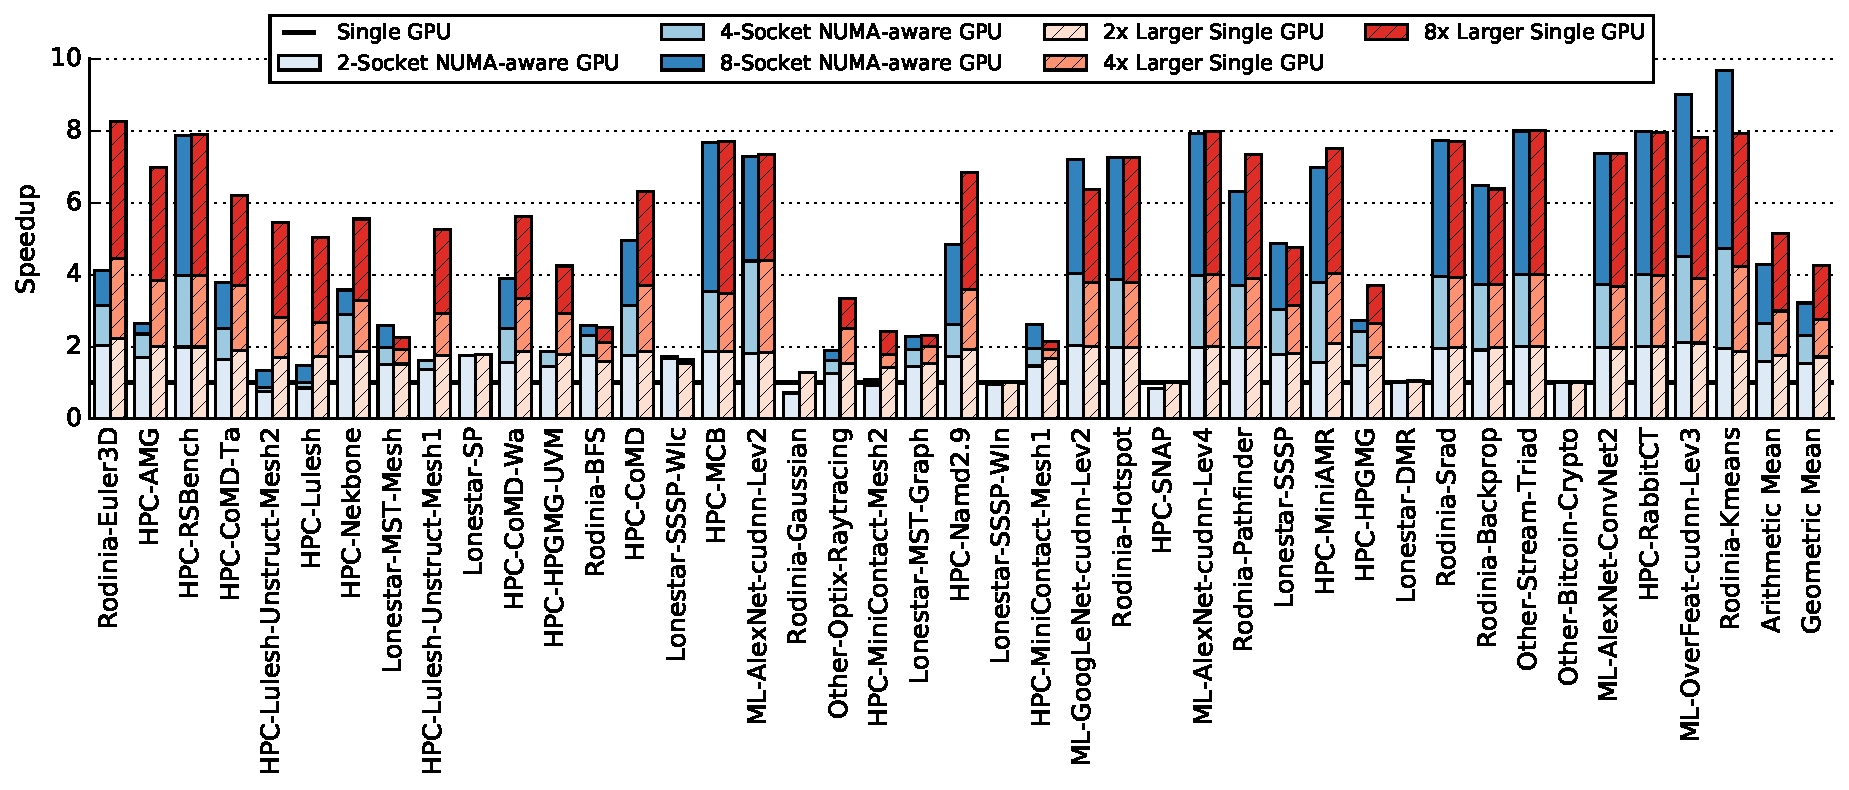
\includegraphics[width=1.0\textwidth]{figures/plot_scalability_mgpu_WB.pdf}
    \caption{Performance scalability of a NUMA-aware GPU compared to theoretical 
    maximum applications performance moving from 1 to 8 GPU sockets.}
    \label{fig:scalability}
    \vspace{-.2in}
\end{figure*}

\section {Discussion}
\label{sec:discussion}
\textbf{Combined Improvement:} Sections~\ref{sec:interconnect} and~\ref{caching} provide two techniques
aimed at more efficiently utilizing scarce NUMA bandwidth within future
NUMA multi-GPU system. These two techniques (interconnect balancing and NUMA-aware
cashing) are orthogonal and can be applied in isolation or combination.  Dynamic 
interconnect balancing has an 
implementation advantage in that the system level changes to enable this feature 
are isolated from the larger GPU design.  Conversely, enabling GPU caching of 
both remote memory and dynamic balancing of cache capacity based on interconnect 
utilization requires changes to both the physical cache architectures and the 
GPU coherence protocol.

Because these two features target similar improvements, when employed together 
their effects are not strictly additive.  Figure~\ref{fig:combined} shows the 
improvement when applying both dynamic interconnects and NUMA-aware cache 
management together.  For benchmarks such as \texttt{CoMD}, these features 
contribute nearly equally to the overall improvement, but for others such as 
\texttt{ML-AlexNet-cudnn-Lev2} or \texttt{HPC-MST-Mesh1}, interconnect 
improvements or caching are the primary contributor respectively.  On average, 
we observe that when combined we see XXX\% a XXX\% improvement over the baseline 
software locality optimized 4-socket NUMA GPU using memory side L2 caches.

\textbf{Scalability:} Ultimately, for vendors to produce multi-socket NUMA GPUs
they must scale efficiently enough for single application customers to see
large enough performance improvements to justify their cost.  To understand
the scalability of this approach Figure~\ref{fig:scalability} shows the
performance of a NUMA-aware multi-socket GPU compared to a single GPU, when
scaled across 2,4, and 8 sockets respectively.  On average a 2 socket NUMA
GPU achieves XXX\% speedup, while 4 sockets and 8 sockets achieve XXX\% speedup
respectively.  Depending on customer expectations these speedups may look attractive
or lackluster, particularly when per-benchmark variance is included.  However,
the scalability of NUMA GPU's is not solely dependent on NUMA GPU microarchitecture.
We observe that for some applications, even if the application was run on much
larger hypothetical single GPUs, performance would not scale.  This may be due to
a variety of reasons beyond NUMA effects, including number of CTA's available, expensive
global synchronizations, or other factors.  Comparing our NUMA-aware GPU implementation
to this hypothetical scaling that applications could achieve, we see that we can
achieve XXX\%, XXX\%, and XXX\% of overall application scalability at 2, 4, and 8 socket
configurations respectively.  This good scaling factor indicates that the NUMA
aspects of future multi-socket GPUs have largely been eliminated as performance limiters
in single GPU application scaling via a NUMA-aware GPU design.

\textbf{Multi-Tenancy of Large GPUs:} In this work we have shown that many 
workloads today have the ability to
saturate (with sufficient parallel work) a GPU that is at least 4$\times$
larger than today's GPUs.  With deep data becoming commonplace across many
computing paradigms, we believe that the trend of having enough computation
to saturate much larger single GPUs will continue into the foreseeable future.
However, when GPUs become larger at the expense of having multiple discrete
GPUs within the system, questions related to GPU provisioning arise.  Applications
that cannot saturate such a GPU will leave resources underutilized and applications
that may be running concurrently in the system currently have to coarse grain
multi-plex the GPU in time cooperatively.  

While not the focus of this work,
there is significant effort in both industry and academia to support finer
grain sharing of GPUs through either shared SM execution~\cite{XXX}, spatial
multi-plexing of a GPU~\cite{XXX}, or through improved time division multiplexing
with GPU pre-emptability~\cite{XXX}.  To support improved per GPU efficiency,
any of these solutions could be applied to a multi-socket GPU to improve utilization
in cases where applications can not fill a significantly larger GPU.  Alternatively,
with additional software work multi-socket GPU designs should be able to be dynamically
partitioned with granularity from 1--N logical GPUs if they are switch connected, providing
yet another level of partitionable flexibility.

\textbf{Power Implications:} \textit{Oreste or Evgeny}
What happens to all the extra bandwidth we need over the interconnect and
power.  we should calculate the extra power but note that even using P2P GPU
access there will still be many remote accesses.  unfortunately we can't quantify
that differential because (drives the point home) there are not multi-GPU versions
for most of our 41 benchmarks.